\usetikzlibrary{trees,shadows}
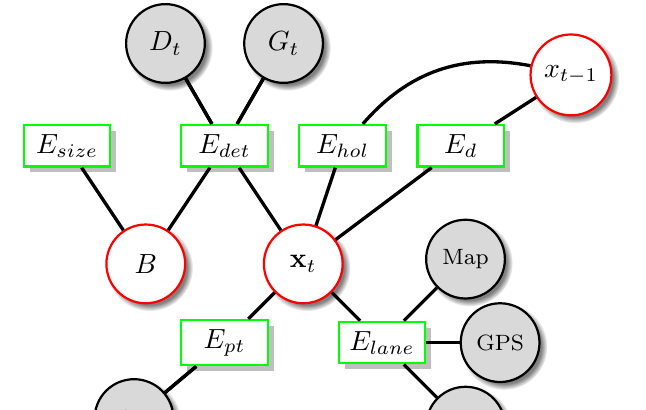
\begin{tikzpicture}[grow cyclic,line width=1.2pt,
    variablenode/.style={circle,circular drop shadow,draw=red,fill=white,thick,minimum width=1.0cm},
    factor/.style={rectangle,drop shadow,draw=green,fill=white,thick,minimum width=1.1cm},
  obs/.style={fill=gray!30,draw=black}]
  \path[use as bounding box] (-4.5, -1.5) rectangle (3,3);
  \path 

  (2.4,2.4) node [variablenode] (xt1) {$x_{t-1}$}
  %(2.6,2.8) node [variablenode] (theta1) {$\theta_{t-1}$}

   (1.0,1.5) node [factor] (fdynx) {$E_{d}$}
  %(1.95,1.8) node [factor,draw=gray,text=gray,minimum width=1cm] (fdynt) {$E_{d}$}

 (-0.5,1.5) node[factor](fhol) {$E_{hol}$}

  %(1, 0)  node[variablenode](theta){$\theta_t$}
  [counterclockwise from=-45,sibling angle=45]
  (0.0, -1.0) node [factor] (flane) {$E_{lane}$} 
  child { node [variablenode,obs] (l) { $L_t$ } }
  child { node [ variablenode,obs,font=\footnotesize] (gps) {GPS}}
  child { node [ variablenode,obs,font=\footnotesize] (gps) {Map}}
  (-1, 0)  node[variablenode](xt){$\mathbf{x}_t$}

  [counterclockwise from=60,sibling angle=60]
  (-2, 1.5) node[factor](fdet){$E_{det}$} 
  child {
    node[variablenode,obs](gp){$G_t$} 
  }
  child {           node[variablenode,obs](Det){$D_t$}
  }

  (-4.0,1.5) node[factor](fsize){$E_{size}$}
  (-3,0) node[variablenode](dim){$B$}
  [counterclockwise from=220]
  (-2.0, -1.0) node[factor](fpt) {$E_{pt}$}
  child { node[variablenode,obs](pt){$u_t$} }


  ;
  \draw (xt) -- (fdet) -- (Det);
  \draw (xt) edge (fpt);
  \draw (fpt) -- (pt);
  %\path  (fpt) edge (theta);
  \draw (fdet) -- (gp);
  \draw (fhol) -- (xt);
  \draw (fhol) edge [bend left] (xt1);
  %\draw (fhol) -- (theta);  	  
  \draw (dim) -- (fdet);
  \draw (fsize) -- (dim);
  %\draw (theta) -- (flane);
  \draw (xt) -- (fdynx) -- (xt1);
  %\draw (theta) -- (fdynt) -- (theta1);
  \draw (xt) -- (flane);
\end{tikzpicture}
